\documentclass[journal]{IEEEtran}
\IEEEoverridecommandlockouts

\usepackage[utf8]{inputenc}
\usepackage[spanish]{babel}
\usepackage{cite}
\usepackage{amsmath,amssymb,amsfonts}
\usepackage{algorithmic}
\usepackage{graphicx}
% Las figuras se citan solo por su nombre. Se buscan en la raíz (carpeta plana, p. ej. Overleaf)
% y en las carpetas del repositorio (docs/diagramas y docs/figuras).
\graphicspath{{./}{../diagramas/}{../figuras/}{../figuras/loao_deauth_to_disas/figures/}{../figuras/loao_disas_to_deauth/figures/}}
\usepackage{textcomp}
\usepackage{xcolor}
\usepackage{tabularx}
\usepackage{xurl}

\newcolumntype{Y}{>{\raggedright\arraybackslash}X}

\makeatletter
\renewcommand{\abstractname}{Resumen}
\renewcommand{\IEEEkeywordsname}{Palabras clave}
\def\abstract{\normalfont
    \if@twocolumn
      \@IEEEabskeysecsize\bfseries\textit{\abstractname.}\relax\ \ignorespaces
    \else
      \bgroup\par\addvspace{0.5\baselineskip}\centering\vspace{-1.78ex}\@IEEEabskeysecsize\textbf{\abstractname}\par\addvspace{0.5\baselineskip}\egroup\quotation\@IEEEabskeysecsize
    \fi\@IEEEgobbleleadPARNLSP}
\def\IEEEkeywords{\normalfont
    \if@twocolumn
      \@IEEEabskeysecsize\bfseries\textit{\IEEEkeywordsname.}\relax\ \ignorespaces
    \else
      \bgroup\par\addvspace{0.5\baselineskip}\centering\@IEEEabskeysecsize\textbf{\IEEEkeywordsname}\par\addvspace{0.5\baselineskip}\egroup\quotation\@IEEEabskeysecsize
    \fi\@IEEEgobbleleadPARNLSP}
\makeatother

\begin{document}

\title{Detección temprana de ataques de desautenticación y disociación en una red Wi-Fi para pequeña empresa mediante aprendizaje automático}

\author{\IEEEauthorblockN{Juan David Quiroga}
\IEEEauthorblockA{\textit{Proyecto Curricular de Ingeniería de Sistemas} \\
\textit{Universidad Distrital Francisco José de Caldas}\\
Bogotá, Colombia \\
jdquirogag@udistrital.edu.co}
}

\maketitle

\begin{abstract}
Este trabajo presenta el diseño y una prueba de concepto para la detección temprana de ataques de desautenticación y disociación en una red Wi-Fi de referencia para una pequeña empresa con 5 a 10 usuarios. La arquitectura se basa en IEEE 802.11ac e incorpora un punto de acceso, segmentación mediante VLAN, un sensor inalámbrico en modo monitor y un servidor de análisis. La prueba de concepto se evaluó con el conjunto de datos AWID3 mediante un flujo en Python, con una partición de tipo \textit{leave-one-attack-out} entre los dos tipos de ataque. Se comparó una línea base basada en umbrales con un Random Forest sobre ventanas temporales de tramas de gestión. En prueba, ambos modelos obtuvieron un F1 entre 0,997 y 1,000; las latencias temporales observadas en los datos fueron de 0,26 s y 1,48 s, distintas del tiempo de procesamiento, que en una reproducción fuera de línea fue de unos pocos milisegundos por ventana. El Random Forest no superó a la línea base. La mitigación se ejecuta como una simulación controlada que solo escribe registros, sin acciones contra redes reales. Los resultados dependen de AWID3, cuyo entorno difiere del escenario de referencia, y de un único episodio de ataque por sentido.

\vspace{1em}
\noindent \textbf{\textit{Abstract.}} This paper presents the design and a proof of concept for early detection of deauthentication and disassociation attacks in a reference Wi-Fi network for a small business with 5 to 10 users. The proposed architecture is based on IEEE 802.11ac and includes an access point, VLAN segmentation, a wireless monitor-mode sensor, and an analysis server. The proof of concept was evaluated with the AWID3 dataset through a Python workflow, using a leave-one-attack-out partition between the two attack types. A threshold-based baseline was compared with a Random Forest model over temporal windows of management frames. On the test set, both models obtained an F1 between 0.997 and 1.000; the observed data-time latencies were 0.26 s and 1.48 s, distinct from processing time, which in an offline replay was a few milliseconds per window. The Random Forest did not outperform the baseline. Mitigation is run as a controlled simulation that only writes records, without actions against real networks. The results depend on AWID3, whose environment differs from the reference scenario, and on a single attack episode per direction.
\end{abstract}

\begin{IEEEkeywords}
Detección temprana, desautenticación, disociación, aprendizaje automático, AWID3, IEEE 802.11, seguridad Wi-Fi. \textbf{\textit{Keywords.}} Early detection, deauthentication, disassociation, machine learning, AWID3, IEEE 802.11, Wi-Fi security.
\end{IEEEkeywords}

\section{Introducción}

Las redes inalámbricas basadas en IEEE 802.11 son un componente habitual de las organizaciones pequeñas. En una startup tecnológica, una interrupción de la conectividad puede afectar el acceso a servicios, la comunicación y la continuidad de las actividades. Entre las amenazas que pueden producir este efecto se encuentran los ataques de denegación de servicio contra las tramas de gestión, incluidos los eventos de desautenticación y disociación.

Kolias \textit{et al.} \cite{kolias2016} estudian las amenazas en redes IEEE 802.11 y las debilidades asociadas al tratamiento de las tramas de gestión. Estos ataques pueden utilizar identidades falsificadas y producir una gran cantidad de eventos en intervalos reducidos. Por esta razón, el monitoreo debe observar el tráfico que circula por el medio inalámbrico y no únicamente los paquetes que llegan al servidor a través de la red cableada.

Las medidas de protección de la infraestructura, como PMF, son necesarias, pero no eliminan la utilidad de la visibilidad y el registro de eventos. En una red donde PMF sea opcional o convivan clientes heredados, un sistema de detección puede aportar información sobre intentos, patrones de tráfico y condiciones de vulnerabilidad. AWID3 constituye una referencia relevante para estudiar ataques contra redes empresariales IEEE 802.11 y sus características de tráfico \cite{chatzoglou2021}; sin embargo, sus condiciones de autenticación y protección no son idénticas a las de una pequeña empresa, por lo que los resultados no se generalizan directamente.

El aprendizaje automático permite comparar patrones de tráfico y construir modelos de clasificación o detección de anomalías. Mishra \textit{et al.} \cite{mishra2019} revisan su aplicación a sistemas de detección de intrusiones, mientras que Zhen \textit{et al.} \cite{zhen2025} discuten sus posibilidades y limitaciones en el análisis de seguridad de redes. En particular, la selección y calidad de las características resulta determinante para evitar modelos que aprendan particularidades del dataset en lugar del comportamiento que se desea detectar \cite{pick2022}.

Este trabajo presenta una prueba de concepto para una red Wi-Fi de referencia de 5 a 10 usuarios. El aporte no es un nuevo algoritmo de aprendizaje, sino la integración de una arquitectura con sensor inalámbrico, una partición diseñada para reducir la fuga de información, una línea base, un modelo supervisado y una evaluación centrada en la latencia temporal de detección. Como se indica en Limitaciones, una ejecución preliminar influyó en la selección final de características; por ello, los resultados se interpretan como exploratorios y no como una estimación completamente independiente. La respuesta de mitigación se ejecuta como una simulación controlada que solo escribe registros, sin enviar tramas ni actuar sobre equipos.

\section{Trabajos relacionados}

Los antecedentes se organizan en cuatro aspectos: detección de intrusiones, calidad de los datos y características, ataques de suplantación y evaluación de ataques de desautenticación.

Mishra \textit{et al.} \cite{mishra2019} presentan una revisión de técnicas de aprendizaje automático para detección de intrusiones. Este trabajo permite justificar la comparación entre una regla de umbral y un modelo supervisado, pero no determina por sí solo la técnica que debe utilizarse en el escenario propuesto.

Alikhanov \textit{et al.} \cite{alikhanov2022} estudian el efecto del muestreo del tráfico sobre métodos de detección basados en aprendizaje automático. Su aporte resulta pertinente para definir las ventanas temporales y documentar cómo las decisiones de observación pueden afectar la latencia y los errores de detección.

Chatzoglou \textit{et al.} \cite{chatzoglou2021} presentan AWID3 y evalúan ataques contra redes empresariales IEEE 802.11. El conjunto se utiliza como fuente de datos de la prueba de concepto, pero se mantiene explícita la brecha entre su entorno y la arquitectura de referencia de una pequeña empresa.

Chatzoglou \textit{et al.} \cite{pick2022} analizan la selección de características y el preprocesamiento en datasets de intrusión 802.11. Este antecedente respalda la necesidad de separar capturas o episodios, evitar la fuga de información y comprobar que las características utilizadas sean comunes al problema de interés.

Aminanto \textit{et al.} \cite{aminanto2018} y Lee \textit{et al.} \cite{impact2020} estudian técnicas de aprendizaje automático y selección de características para clases de suplantación etiquetadas en AWID. Estos trabajos se utilizan como antecedentes de modelado y análisis de características, no como evidencia específica de que \texttt{wlan.seq} o la potencia de señal permitan identificar por sí solos tramas falsificadas de desautenticación.

Milliken \textit{et al.} \cite{milliken2013} analizan el efecto de la selección de métricas en el desempeño de ataques de desautenticación. Este resultado motiva una separación entre las características de entrada del modelo y las métricas de evaluación, especialmente la latencia, la tasa de falsas alertas y la detección por episodio.

Finalmente, Halbouni \textit{et al.} \cite{halbouni2023} revisan WPA3 y sus problemas de seguridad. Esta referencia se utiliza para discutir la evolución futura hacia WPA3 y PMF, sin confundir la activación de PMF con una migración obligatoria hacia IEEE 802.11ax.

\section{Metodología}

El componente analítico se organiza mediante CRISP-DM, mientras que el diseño de red sigue un flujo descendente de ingeniería: requisitos, arquitectura, conectividad, segmentación, seguridad, monitoreo e integración con el análisis. La evaluación se realizó sobre AWID3 en modo fuera de línea; los resultados se presentan en la sección de resultados. La Figura~\ref{fig:pipeline} resume las fases de CRISP-DM y los módulos de cada una.

\begin{figure*}[t]
\centering
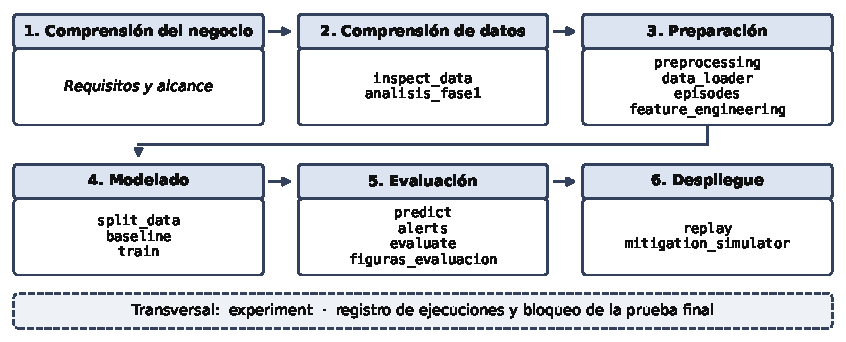
\includegraphics[width=0.85\textwidth]{pipeline-crisp-dm.pdf}
\caption{Flujo de trabajo según CRISP-DM y módulos de cada fase. El módulo \texttt{experiment} registra cada ejecución y bloquea la repetición de la prueba final.}
\label{fig:pipeline}
\end{figure*}

\subsection{Comprensión del contexto y objetivos}

El escenario corresponde a una pequeña empresa con entre 5 y 10 usuarios y una red Wi-Fi principal basada en IEEE 802.11ac. El objetivo analítico es detectar tempranamente eventos asociados con desautenticación y disociación en tramas de gestión.

El alcance se define por tipo de trama: la etiqueta de AWID3 identifica el ataque de desautenticación (\texttt{Deauth}) y el de disociación (\texttt{Disas}), sin separar tramas de difusión de tramas dirigidas. La proporción de tramas de difusión dentro de cada tipo se reporta como análisis complementario.

La detección temprana se define como la generación de una alerta después del inicio registrado del evento y antes de que se observen todas sus tramas. La prueba no afirma una predicción previa a la primera trama maliciosa.

\subsection{Comprensión de los datos}

AWID3 contiene 745 archivos CSV con 254 columnas idénticas. Para esta prueba de concepto se usaron dos capturas: \texttt{cap\_a}, con los archivos de desautenticación, y \texttt{cap\_b}, con los de disociación. Cada captura dura unos 600 s. El ataque ocupa unos 180 s: en \texttt{cap\_a} hay 38\,942 tramas de ataque sobre 1\,626\,469 tramas, y en \texttt{cap\_b}, 75\,131 sobre 2\,013\,716. El tráfico normal ocupa el inicio de la captura y el ataque forma un único bloque continuo al final. Esta geometría determina la partición (sección de partición y episodios).

\begin{table*}[t]
\caption{Mapeo de columnas de AWID3 a campos internos. La columna \texttt{mfpr} no existe en el CSV y se omite.}
\label{tab:mapeo}
\centering
\footnotesize
\begin{tabularx}{\textwidth}{p{2.6cm}p{6.2cm}Y}
\hline
Campo interno & Columna AWID3 & Uso \\
\hline
\path{ts} & \path{frame.time_epoch} & Ventanas y latencia temporal \\
\path{fc_type} & \path{wlan.fc.type} & Tipo de trama; se combina con el subtipo para identificar desconexiones \\
\path{fc_subtype} & \path{wlan.fc.subtype} & Subtipo de trama; 10 o 12 junto con tipo 0 \\
\path{src}, \path{dst}, \path{bssid} & \path{wlan.sa}, \path{wlan.da}, \path{wlan.bssid} & Identificadores anonimizados; se conserva el destino de difusión \\
\path{reason_code} & \path{wlan.fixed.reason_code} & Entrada para los conteos \path{rc_7}, \path{rc_1} y \path{rc_other} \\
\path{seq} & \path{wlan.seq} & Entrada para \path{seq_jump_max} \\
\path{signal_dbm} & \path{radiotap.dbm_antsignal} & Entrada para \path{signal_std_disconn} \\
\path{protected} & \path{wlan.fc.protected} & Entrada para \path{frac_protected_mgmt} \\
\path{mfpc} & \path{wlan.rsn.capabilities.mfpc} & No es característica del modelo (casi nulo); la mitigación simulada lo usa en las tramas de (re)asociación \\
\path{label} & \path{Label} & Etiqueta de referencia: Deauth, Disas o Normal \\
\hline
\end{tabularx}
\end{table*}

Los campos de protección tienen cobertura desigual. El campo \texttt{wlan.rsn.capabilities.mfpc} existe, pero solo tiene valor en menos del 0,5 \% de las tramas. Ese valor aparece en las tramas de (re)asociación, no en el resto, y es el que usa la mitigación simulada. El campo \texttt{mfpr} no está presente en el CSV, así que la exigencia de PMF por parte del punto de acceso no se puede conocer y un cliente sin observación previa se trata como de compatibilidad desconocida. En la muestra revisada, las capturas corresponden a 5 GHz, canal 36 (5180 MHz), y no se observó diversidad de canal.

Las desconexiones de gestión etiquetadas como normales son muy pocas: 72 en \texttt{cap\_a} (69 de subtipo 10 y 3 de subtipo 12) y 51 en \texttt{cap\_b} (45 y 6). Las tramas con los mismos números de subtipo pero de tipo control o datos no son desautenticaciones. Esta distinción es la que permite definir la desconexión a partir de \texttt{fc\_type} y \texttt{fc\_subtype} juntos.

La marca temporal de las tramas de ataque de gestión es entera en el 100 \% de los casos. Esta propiedad no es exclusiva del ataque: en tramas de gestión normales de acción (subtipo 13) la fracción entera llega a 0,96 en \texttt{cap\_a} y a 0,999 en \texttt{cap\_b}. Por esta razón la fracción de la marca temporal no se usa como señal de clase, y las características derivadas de intervalos entre tramas se retiran (sección de características).

\subsection{Preparación y características}

Los registros se convierten a un formato interno con marca temporal, captura, tipo y subtipo, identificadores anonimizados, código de motivo, secuencia, señal y protección, cuando estos campos existen. Las direcciones MAC se anonimizan con HMAC-SHA256 truncado a 12 caracteres hexadecimales, usando una sal que se lee desde una variable de entorno y no se guarda en el repositorio. La difusión se conserva como destino especial. Los datos originales se mantienen separados de los procesados y no se modifican.

El código de motivo se almacena como entero de 32 bits. Un entero de 16 bits con signo llega solo hasta 32 767, mientras que AWID3 contiene códigos de hasta 65 535; al convertirlos a 16 bits los valores fuera de rango se corrompen sin aviso.

Se usan ventanas deslizantes de duración $W = 5$ s y paso $S = 1$ s, con $k=1$: una ventana es de ataque si contiene al menos una trama etiquetada del evento. La resolución del dato es de 1 s, así que un paso menor no añade precisión real. La verificación con datos de entrenamiento confirma que el 100 \% de las ventanas de ataque contienen al menos una trama de desconexión de gestión (130 de 130 en deauth$\rightarrow$disas y 97 de 97 en disas$\rightarrow$deauth), lo que respalda la duración elegida.

Las características de cada ventana se seleccionan con una lista permitida. Esa lista incluye el número de tramas totales, de gestión y de datos, su razón, el número de desconexiones y su tasa, la variación entre ventanas, la fracción de tramas de gestión protegidas, los conteos por código de motivo (\texttt{rc\_7}, \texttt{rc\_1} y \texttt{rc\_other}), la mayor diferencia de secuencia entre tramas de una misma fuente y la desviación de la señal de las desconexiones. El perfil que usan los experimentos principales de caso C es un subconjunto de esa lista: excluye los conteos por subtipo, \texttt{rc\_7} y \texttt{rc\_1}, las fuentes y destinos únicos de las desconexiones y la fracción de difusión. Quedan 11 características: número de tramas totales, de gestión y de datos, razón entre datos y gestión, número de desconexiones, su tasa y su variación entre ventanas, fracción de gestión protegida, \texttt{rc\_other}, la mayor diferencia de secuencia y la desviación de la señal. El conjunto se fijó antes de la evaluación final.

\begin{table*}[htbp]
\caption{Características del perfil de caso C (11 columnas). $W$ es la duración de la ventana. Las columnas \texttt{n\_deauth}, \texttt{n\_disas}, \texttt{rc\_7}, \texttt{rc\_1}, \texttt{frac\_broadcast\_dst\_disconn} y \texttt{n\_unique\_*} están excluidas del perfil de caso C.}
\label{tab:caracteristicas}
\centering
\footnotesize
\begin{tabularx}{\textwidth}{p{4.5cm}Y}
\hline
Característica & Definición \\
\hline
\path{n_frames_total} & Número de tramas de la ventana. \\
\path{n_mgmt}, \path{n_data} & Tramas de gestión (tipo 0) y de datos (tipo 2). \\
\path{ratio_data_mgmt} & \path{n_data} dividido entre máx(\path{n_mgmt}, 1). \\
\path{n_disconn} & Desconexiones de gestión: tipo 0 y subtipo 10 o 12. \\
\path{rate_disconn} & \path{n_disconn} dividido entre $W$. \\
\path{delta_n_disconn} & \path{n_disconn} de la ventana menos el de la ventana anterior. Nulo en la primera ventana. \\
\path{frac_protected_mgmt} & Fracción de tramas de gestión con \path{protected} = 1. \\
\path{rc_other} & Desconexiones cuyo código de motivo no es 7 ni 1. \\
\path{seq_jump_max} & Mayor salto de \path{seq}, en aritmética módulo 4096, entre tramas de gestión consecutivas de una misma fuente que emitió desconexiones. \\
\path{signal_std_disconn} & Desviación estándar de la señal (dBm) de las desconexiones, si hay al menos dos. \\
\hline
\end{tabularx}
\end{table*}

Las características \path{iat_disconn_mean}, \path{iat_disconn_std} e \path{iat_disconn_min} se retiraron. En las ventanas normales hay menos de dos desconexiones, así que estos valores son nulos y se imputan con $-1$. Ese valor señala la clase normal casi sin error, así que la característica filtra la etiqueta por un mecanismo de imputación. El truncado de la marca temporal que se había previsto para estas características no tiene efecto sobre las características usadas.

Las fuentes y destinos únicos de las desconexiones y la fracción de difusión se excluyen del perfil de caso C porque difieren de forma clara entre ataques en el conjunto de entrenamiento: en el sentido deauth$\rightarrow$disas, la cantidad de fuentes únicas es 2,64 en ataque y 0,01 en normal. La verificación se hizo solo con las capturas de entrenamiento para no usar información de la prueba. Los conteos por subtipo y los códigos \texttt{rc\_7} y \texttt{rc\_1} se excluyen porque actúan como sustitutos del subtipo.

\subsection{Partición y episodios}

Un episodio es una ráfaga de tramas objetivo separada de otra por un silencio superior a $T$. En AWID3 cada captura tiene un único episodio, y la brecha máxima entre tramas objetivo es de 1 s. Por esa razón $T$ se fija en 2 s. El método basado en percentiles de los intervalos daría un valor degenerado, porque casi todos los intervalos valen cero.

La partición tradicional de tres vías no es viable con esta geometría. Con cortes por cuantil de las tramas de ataque, los conjuntos de validación y prueba quedan formados solo por ataque, sin ventanas normales, y la partición se rechaza. Por eso se usa \textit{leave-one-attack-out} (caso C) como partición principal, en ambos sentidos: se entrena y valida con la captura de un ataque y se prueba con la captura completa del otro.

La validación de cada sentido se ubica sobre la frontera entre el tráfico normal y el ataque, de modo que contenga ambos tipos de tramas. Como hay una sola frontera por captura, el entrenamiento se divide en dos unidades: el tráfico normal inicial y el tramo final del ataque, ambos separados de la validación por una purga de 10 s. La purga es igual a la mayor ventana de sensibilidad, según la regla de que la purga sea al menos $W$. La captura de prueba se usa completa, incluido su inicio. Esto hace que la latencia sea medible en prueba. Para el sentido deauth$\rightarrow$disas, el entrenamiento tiene 503 ventanas, la validación 66 y la prueba 600; para disas$\rightarrow$deauth, 465, 105 y 599. En ambos sentidos los tres conjuntos contienen ventanas normales y de ataque. La validación empieza 36 s antes del inicio del ataque y termina 35 s después en deauth$\rightarrow$disas y 74 s después en disas$\rightarrow$deauth, porque el ataque de disociación dura más y la franja se calcula como fracción de la duración del ataque; el entrenamiento queda a ambos lados con purga de 10 s (Tabla~\ref{tab:parametros}).

\subsection{Modelado}

La línea base alerta cuando \texttt{n\_disconn} alcanza un umbral $\theta$. El umbral se elige en validación por máximo F1 por ventana, y en caso de empate se toma el menor. El Random Forest usa 11 características (ver sección de características). Su búsqueda explora 12 combinaciones de \texttt{n\_estimators} (100 y 300), \texttt{max\_depth} (sin límite, 10 y 20) y \texttt{min\_samples\_leaf} (1 y 5), con pesos de clase equilibrados. El umbral del Random Forest se elige también en validación, por máximo F1. La imputación de valores nulos es constante e igual a $-1$. Ninguna decisión usa el conjunto de prueba.

Regla de alerta. El modelo alerta en una ventana cuando su puntuación alcanza el umbral. Las ventanas de alerta consecutivas de una misma captura se fusionan en un solo evento si la separación entre sus instantes finales no supera \texttt{max\_gap} = 1 s. El evento conserva el instante de la primera ventana, que es el instante de alerta del protocolo.
\begin{table*}[t]
\caption{Parámetros congelados de los experimentos de caso C.}
\label{tab:parametros}
\centering
\footnotesize
\begin{tabularx}{\textwidth}{p{4.1cm}Y}
\hline
Parámetro & Valor \\
\hline
Ventana $W$ y paso $S$ & 5 s y 1 s (sensibilidad: 3 s y 10 s) \\
Tipo de ventana $k$ & 1 (de ataque si contiene una trama de ataque) \\
Separación de episodios $T$ & 2 s, fijo \\
Unión de alertas \path{max_gap} & 1 s \\
Purga & 10 s a cada lado de cada corte \\
Validación (caso C) & Desde 36 s antes del inicio del ataque hasta 35 s después (deauth$\rightarrow$disas) o 74 s después (disas$\rightarrow$deauth) \\
Umbral & Máximo F1 por ventana en validación; en empate, el menor \\
Línea base & Alerta si \path{n_disconn} $\geq \theta$ \\
Random Forest & 12 combinaciones: \path{n_estimators} $\in \{100, 300\}$, \path{max_depth} $\in \{\text{sin límite}, 10, 20\}$ y \path{min_samples_leaf} $\in \{1, 5\}$; pesos de clase equilibrados \\
Imputación & Constante $-1$ \\
Semilla & 42 \\
\hline
\end{tabularx}
\end{table*}

Isolation Forest no se evaluó. El plan lo condiciona a que la exploración demuestre que la detección no supervisada es viable, y la exploración no llegó a esa comparación. No se implementaron aprendizaje por refuerzo, aprendizaje federado ni redes neuronales profundas.

\section{Diseño de la solución}

La arquitectura de referencia estará compuesta por clientes inalámbricos, un punto de acceso, un switch con soporte 802.1Q, un router o gateway, un sensor inalámbrico en modo monitor y un servidor de análisis.

El AP operará en 5 GHz bajo IEEE 802.11ac, con un canal de referencia 36 y un ancho inicial de 40 MHz. La red corporativa utilizará la VLAN 10 con el segmento \texttt{192.168.10.0/24}; la gestión del AP, sensor y servidor utilizará la VLAN 20 con \texttt{192.168.20.0/24}; y los invitados utilizarán la VLAN 30 con \texttt{192.168.30.0/24}.

El AP y el router se conectarán al switch mediante enlaces troncales 802.1Q que transportarán las VLAN 10, 20 y 30. El sensor y el servidor se conectarán mediante puertos de acceso en la VLAN 20. El router funcionará mediante un esquema \textit{router-on-a-stick}, realizará el enrutamiento inter-VLAN y aplicará las ACL. La VLAN 30 tendrá únicamente salida a Internet y no podrá acceder a las VLAN 10 ni 20. El acceso a la VLAN 20 se restringirá a comunicaciones administrativas autorizadas. Una lista de control de acceso sin estado, como la que se verifica a nivel lógico en la topología de referencia, no distingue las respuestas de conexiones iniciadas desde la red corporativa; el diseño real debe permitir únicamente respuestas de conexiones establecidas o usar un cortafuegos con estado.

\begin{table}[htbp]
\caption{Plan de VLAN y direccionamiento de la topología de referencia. La puerta de enlace es la dirección \texttt{.1} de cada red.}
\label{tab:vlan}
\centering
\footnotesize
\begin{tabularx}{\columnwidth}{llY}
\hline
VLAN & Red & Equipos \\
\hline
10 Corporativa & \texttt{192.168.10.0/24} & 3 PC (\texttt{.10}--\texttt{.12}) \\
20 Gestión & \texttt{192.168.20.0/24} & Servidor (\texttt{.20}), sensor (\texttt{.10}) \\
30 Invitados & \texttt{192.168.30.0/24} & PC (\texttt{.10}) \\
\hline
\end{tabularx}
\end{table}

\begin{figure*}[t]
\centering
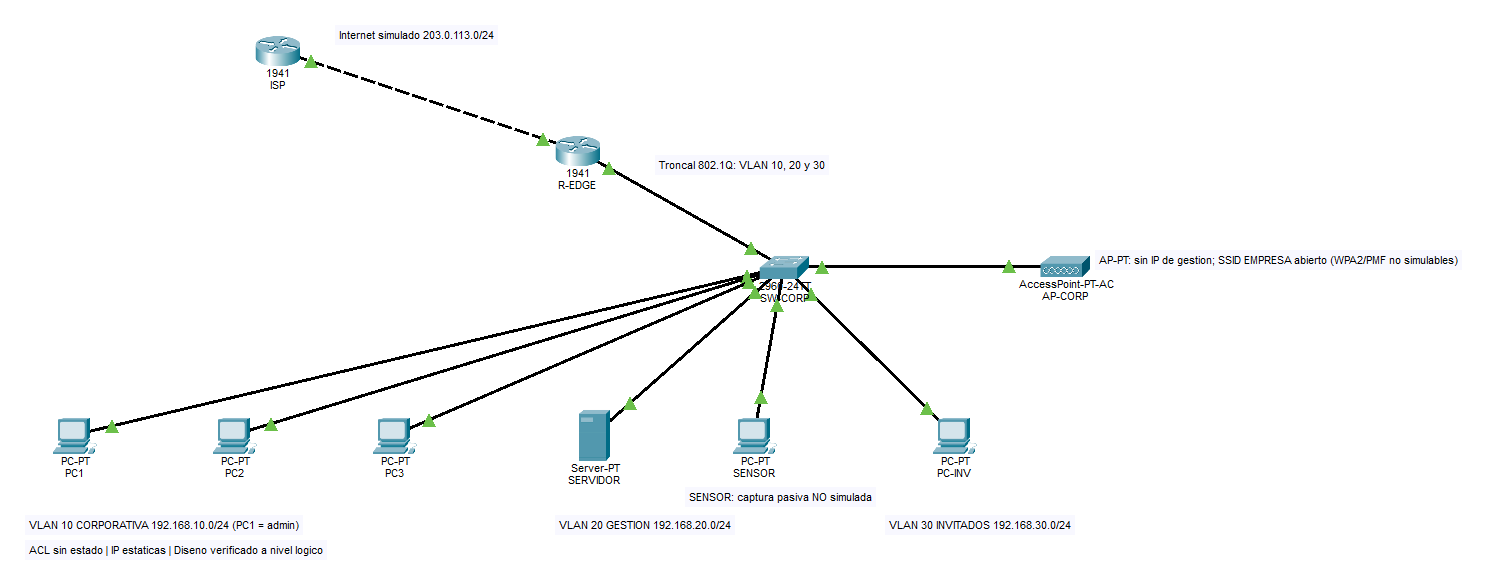
\includegraphics[width=0.92\textwidth]{topologia-empresa.png}
\caption{Topología de referencia construida y verificada a nivel lógico en Cisco Packet Tracer 9.0.1. El router \texttt{ISP} representa Internet con la red \texttt{203.0.113.0/24}, reservada para documentación. La captura pasiva del sensor y la seguridad inalámbrica no se simulan.}
\label{fig:topologia}
\end{figure*}

La topología se construyó en Cisco Packet Tracer 9.0.1 y se verificó a nivel lógico (Figura~\ref{fig:topologia} y Tabla~\ref{tab:vlan}) con diez pruebas de conectividad. Los equipos de una misma VLAN y el sensor con el servidor se comunican. Los invitados alcanzan su puerta de enlace y el router de salida, con traducción de direcciones (configurada para las tres VLAN y observada en el tráfico de los invitados), pero no las VLAN 10 ni 20. Solo la estación administrativa de la VLAN 10 alcanza la VLAN 20; los demás equipos de la VLAN 10 no, y Packet Tracer informa que el router descarta el paquete por la regla de la ACL de gestión. Esta verificación no valida la capa inalámbrica: Packet Tracer no simula el enlace 802.11ac ni el modo monitor. Su punto de acceso no admite dirección IP de gestión ni etiquetado 802.1Q y queda abierto, por lo que WPA2 con PMF opcional, el canal 36 y el ancho de 40 MHz siguen siendo supuestos de diseño. El sensor se representa como un equipo cableado, y no se simulan DHCP ni DNS.

El sensor capturará pasivamente el tráfico del aire en modo monitor y reenviará registros o características al servidor. Esta función no puede ser reemplazada por un servidor conectado detrás del router, porque las tramas de gestión no necesariamente atraviesan la red cableada.

El sensor calcula las características de cada ventana con la misma función que el análisis en lote y envía al servidor un mensaje por cada ventana cerrada, es decir, uno por paso $S = 1$ s, en lugar de las tramas capturadas. Cada mensaje es un objeto JSON en una sola línea, enviado por una conexión TCP persistente que inicia el sensor hacia el servidor, con un puerto no privilegiado configurable (por ejemplo, el 5140). Los dos equipos están en la VLAN 20, así que el tráfico no atraviesa el router ni sus ACL. El mensaje contiene la versión del formato, un identificador neutro del sensor, el número de ventana, el instante de cierre, $W$, $S$ y las 11 características del perfil; ninguna de ellas contiene direcciones MAC, y el mensaje no lleva etiquetas ni tipo de ataque. Un mensaje de ejemplo construido con una ventana real ocupa unos 310 bytes, es decir, unos 2,5 kbit/s a un mensaje por segundo, frente a entre 2\,700 y 3\,300 tramas por segundo en las capturas. El servidor aplica el modelo y genera las alertas. En un despliegue real el canal debería ir cifrado y autenticado en ambos extremos (por ejemplo, TLS con certificados de cliente), porque un mensaje falso podría provocar o suprimir alertas. Este canal es una decisión de diseño: no está implementado ni medido, y en Packet Tracer la conexión entre el sensor y el servidor es solo lógica. Además, la lista de clientes de la mitigación simulada necesita las observaciones de (re)asociación, que este formato de mensaje no incluye.

Como estimación de diseño, un AP 802.11ac 2x2 en 40 MHz puede ofrecer cerca de 400 Mbps de tasa física en condiciones favorables. Considerando una eficiencia útil aproximada del 50 \%, se utilizan 200 Mbps como capacidad agregada de referencia, equivalente a unos 20 Mbps por usuario con 10 usuarios activos. Estas cifras son supuestos de planificación: no se apoyan en una fuente bibliográfica ni en una medición física, y ningún resultado de este trabajo depende de ellas.

La seguridad de referencia considera WPA2-Personal con PMF opcional o coexistencia de clientes heredados. La evolución futura considera WPA3-Personal con PMF requerido. PMF y la migración a IEEE 802.11ax se tratan como decisiones independientes.

La configuración inalámbrica objetivo es la siguiente. El punto de acceso publicaría dos SSID: uno corporativo, asociado a la VLAN 10, y uno de invitados, asociado a la VLAN 30. Ambos usarían WPA2-Personal con cifrado AES-CCMP, claves precompartidas distintas y WPS desactivado. Las PMF (IEEE 802.11w) estarían en modo opcional: los clientes que las soportan las negocian y los heredados siguen pudiendo asociarse. La gestión del punto de acceso quedaría en la VLAN 20. Esta decisión es la que da sentido al detector: un cliente que no negocia PMF no está protegido frente a tramas de desautenticación y disociación falsificadas, y las PMF no protegen las tramas anteriores a que se establezcan las claves. Exigir PMF mediante WPA3-Personal eliminaría la compatibilidad con los clientes heredados. Cisco Packet Tracer no permite configurar WPA2 ni PMF en su punto de acceso ni en sus clientes inalámbricos, de modo que esta configuración es un supuesto de diseño que no se verificó en la topología.

\section{Implementación de la prueba de concepto}

La implementación se realiza en Python con Pandas, NumPy, Scikit-learn y Matplotlib. Los scripts de análisis de la fase de inspección se mantienen fuera del flujo principal, y el código cuenta con pruebas automatizadas (114 en esta versión).

El flujo implementado y su estado en esta versión son los siguientes:

\begin{enumerate}
    \item Inspección de los archivos y generación de un informe de estructura. \textit{Implementado.}
    \item Limpieza y normalización de los datos. \textit{Implementado.}
    \item Anonimización de identificadores. \textit{Implementado.}
    \item Construcción de episodios y ventanas temporales. \textit{Implementado.}
    \item Extracción de características. \textit{Implementado.}
    \item Definición de entrenamiento, validación y prueba sin fuga de información. \textit{Implementado con partición de caso C.}
    \item Ejecución de la línea base. \textit{Implementado.}
    \item Entrenamiento y almacenamiento del Random Forest. \textit{Implementado.}
    \item Predicción sobre datos reservados. \textit{Implementado.}
    \item Generación de alertas estructuradas. \textit{Implementado.}
    \item Reproducción temporal para medir el tiempo de procesamiento y verificar que coincide con el cálculo en lote. \textit{Implementado y ejecutado sobre la prueba final.} La latencia de detección reportada sigue siendo la de los datos; el tiempo de procesamiento se informa aparte.
    \item Ejecución de la mitigación simulada. \textit{Implementado y ejecutado sobre la prueba final;} solo escribe registros.
    \item Figuras de evaluación a partir de resultados ya guardados. \textit{Implementado;} el \textit{script} solo lee, no repite la prueba.
\end{enumerate}

\begin{table*}[t]
\caption{Componentes y actividades del flujo organizados por fase de CRISP-DM.}
\label{tab:modulos}
\centering
\footnotesize
\begin{tabularx}{\textwidth}{p{3.6cm}p{5.4cm}Y}
\hline
Fase CRISP-DM & Módulo o componente & Función o estado \\
\hline
Comprensión del negocio & Requisitos y alcance & Contexto de 5 a 10 usuarios, objetivo de disponibilidad y límites de la prueba \\
Comprensión de datos & \path{inspect_data}, \path{analisis_fase1} & Estructura y etiquetas; el segundo es un script de apoyo \\
Preparación & \path{preprocessing}, \path{data_loader} & Formato interno, tipos y anonimización \\
Preparación & \path{episodes}, \path{feature_engineering} & Episodios, rejilla de ventanas y características \\
Modelado & \path{split_data}, \path{baseline}, \path{train} & Partición congelada, línea base y Random Forest \\
Evaluación & \path{predict}, \path{alerts}, \path{evaluate} & Puntuaciones, alertas, métricas y latencia temporal \\
Evaluación & \path{figuras_evaluacion} & Figuras desde resultados guardados; solo lectura \\
Despliegue & \path{replay}, \path{mitigation_simulator} & Reproducción temporal verificada contra el lote y mitigación simulada; ejecutados sobre la prueba final \\
Transversal & \path{experiment} & Registro de ejecuciones y guardas de R6 y R10 \\
\hline
\end{tabularx}
\end{table*}

Entorno y reproducibilidad. El código se ejecuta con Python 3.13 y las versiones fijadas en \texttt{requirements.txt} (pandas 3.1.0, NumPy 2.4.6, scikit-learn 1.9.1 y pyarrow 26.0.0, entre otras). Cada experimento guarda su configuración, su semilla, el commit del código y el estado del árbol de trabajo. Los resultados de detección y de latencia corresponden al commit \texttt{6a49bb4}, marcado con la etiqueta \texttt{gate-d}; la reproducción temporal y la mitigación simulada se ejecutaron sobre el commit \texttt{545bf2e}, cuyo único cambio en código y configuración respecto de \texttt{6a49bb4} es un comentario de documentación. Los comandos para regenerar cada salida están en \texttt{README.md}.

Cada ejecución de prueba queda registrada con el commit del código, el estado del árbol de trabajo y un marcador que impide repetirla. La partición congelada guarda su propio commit.

La mitigación simulada registra la hora de la alerta, el tipo de evento, la puntuación, la acción representada y el resultado. No envía tramas de desautenticación ni ejecuta acciones contra equipos reales. Una notificación agrupa las alertas que llegan dentro del enfriamiento de 30 s, y la prioridad es alta cuando la puntuación supera 0,9; ambos valores son supuestos de simulación y no se optimizaron. Los clientes se listan como compatibles con PMF, no compatibles o de compatibilidad desconocida según el campo \texttt{mfpc} observado antes de la alerta, y nunca se aísla una fuente por su dirección MAC. El cambio de canal y la localización aproximada por RSSI se registran solo como acciones de diseño.

\section{Protocolo de evaluación}

La detección se evalúa mediante matriz de confusión, precisión (\textit{precision}), exhaustividad (\textit{recall}), F1, falsos positivos, falsos negativos y falsas alertas por hora de tráfico normal.

Como referencia de diseño se adoptan tres criterios de aceptación: latencia de detección de hasta 2 s, como máximo una falsa alerta por hora de tráfico normal y F1 por ventana de al menos 0,90. Son criterios propuestos por el autor y se fijaron después de observar resultados preliminares; por tanto, no son umbrales previos a la experimentación y no se usaron para elegir el modelo ni sus parámetros.

La detección temprana se evalúa por episodio mediante la primera alerta, la latencia desde el primer evento registrado y el número de episodios detectados. Un episodio se considera detectado si existe una ventana de alerta cuyo instante final es posterior al inicio del episodio y cuyo inicio no es posterior al final del episodio más $W$. La latencia es el instante final de la primera de esas ventanas menos el inicio del episodio. Se calcula con las marcas temporales de las tramas, no con el tiempo de procesamiento, y solo cuando el episodio conserva su inicio completo en el conjunto evaluado. Cuando el conjunto de prueba no conserva el inicio completo, la latencia se reporta como no disponible.

El rendimiento operativo se mide reproduciendo las tramas de la captura de prueba en orden temporal, con el mismo cálculo de características que el procesamiento en lote: se registra el tiempo de procesamiento por ventana, desde el registro hasta la predicción, y la tasa de procesamiento frente a la tasa de entrada. La reproducción solo se acepta si sus decisiones coinciden ventana a ventana con las del lote. No se reportan como resultados reales la reconexión, la continuidad del servicio ni el impacto sobre usuarios, porque no existe hardware físico.

En la ejecución final, las decisiones de ajuste se tomaron solo con los conjuntos de entrenamiento y validación. Sin embargo, una ejecución preliminar sobre prueba influyó en la selección final de características; por ello, aunque esa ejecución se descartó y se documenta en Limitaciones, la estimación final no debe considerarse completamente independiente del proceso de selección.

\section{Resultados}

La Tabla~\ref{tab:resultados} resume el rendimiento en prueba. En el sentido deauth$\rightarrow$disas, el modelo se entrena y valida con la captura de desautenticación y se prueba con la captura de disociación; el sentido inverso es simétrico. Las cifras de detección y latencia provienen de los registros de la ejecución final, atada al commit \texttt{6a49bb4}; las de reproducción temporal, de la ejecución sobre el commit \texttt{545bf2e}.

\begin{table*}[htbp]
\caption{Resultados en prueba con partición de caso C. En cada sentido se entrena y valida con una captura y se prueba con la otra completa. Precisión igual a 1,000 en las cuatro filas. FA/h: falsas alertas por hora de tráfico normal.}
\label{tab:resultados}
\centering
\begin{tabular}{llcccc}
\hline
Modelo & Sentido (entrenamiento $\rightarrow$ prueba) & F1 & Recall & Latencia (s) & FA/h \\
\hline
Random Forest & deauth $\rightarrow$ disas & 0,9973 & 0,9946 & 0,262 & 0 \\
Random Forest & disas $\rightarrow$ deauth & 0,9972 & 0,9944 & 1,483 & 0 \\
Umbral $n\_disconn$ & deauth $\rightarrow$ disas & 1,0000 & 1,0000 & 0,262 & 0 \\
Umbral $n\_disconn$ & disas $\rightarrow$ deauth & 0,9972 & 0,9944 & 1,483 & 0 \\
\hline
\end{tabular}
\end{table*}

En el sentido deauth$\rightarrow$disas, el Random Forest detecta 185 de las 186 ventanas de ataque y no produce falsos positivos. La línea base detecta las 186. La diferencia es una sola ventana. En disas$\rightarrow$deauth, ambos modelos tienen el mismo resultado. La latencia coincide en los dos modelos, porque la primera alerta de ambos ocurre en el mismo instante.

En la prueba de deauth$\rightarrow$disas, la ventana de ataque con menos desconexiones tiene 82 tramas, mientras que la ventana normal con más tiene 1; en ese sentido, el conteo de desconexiones por sí solo separa las clases observadas. La importancia por permutación del Random Forest en validación es cero para todas las características. Este resultado no demuestra que varias características separen por sí solas: puede deberse a redundancia, a la saturación de la métrica o al procedimiento de cálculo, y requeriría un análisis de ablación para interpretarse. La conclusión respaldada por la comparación es que, en este conjunto, el Random Forest no aporta una mejora medible frente a la regla de umbral sobre \texttt{n\_disconn}.

El análisis de sensibilidad se hizo solo en validación. Con ventanas de 3 s, 5 s y 10 s, el F1 es 1,000 en los tres casos. También es 1,000 el modelo sin códigos de motivo, lo que indica que la detección no depende de \texttt{rc\_7}, el código más asociado al ataque. Estas cifras se basan en 66 ventanas de validación en el modelo principal y en el modelo sin códigos de motivo, 68 con $W=3$ s y 61 con $W=10$ s, y solo en el sentido deauth$\rightarrow$disas, así que solo indican robustez de forma preliminar.

La latencia de 0,26 s y de 1,48 s se obtiene de un único episodio por sentido. No es posible estimar media, dispersión ni intervalo de confianza.

\begin{figure*}[t]
\centering
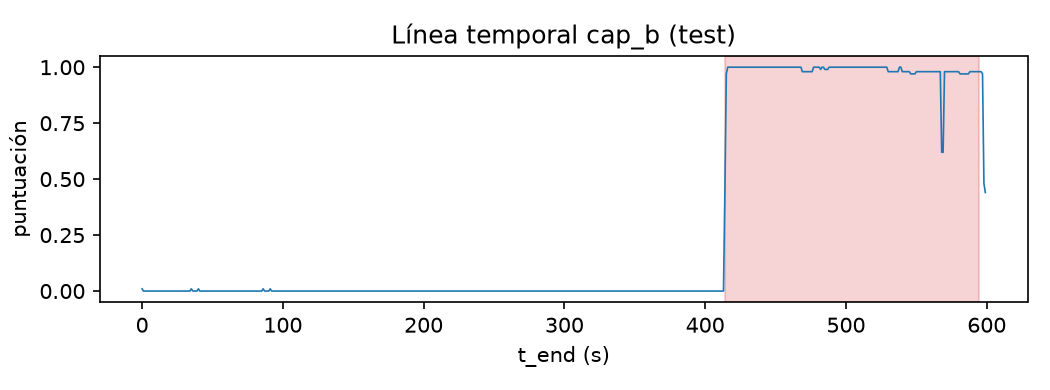
\includegraphics[width=0.48\textwidth]{timeline_cap_b_test.png}\hfill
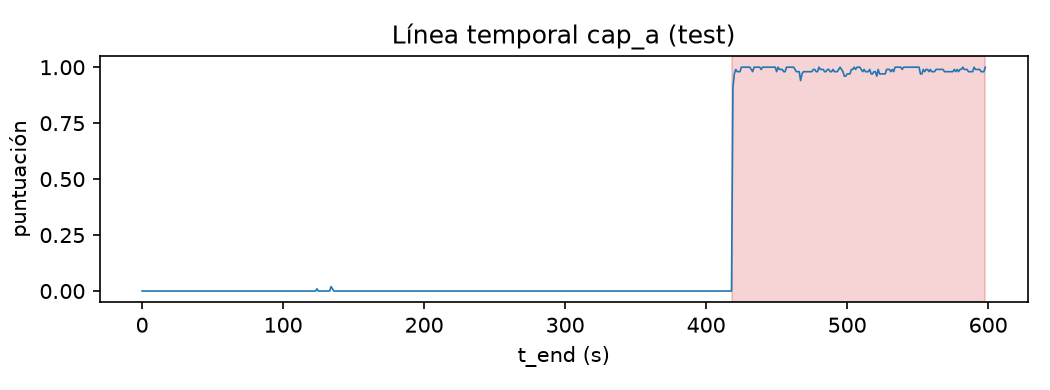
\includegraphics[width=0.48\textwidth]{timeline_cap_a_test.png}
\caption{Puntuación del Random Forest por ventana en la captura de prueba; a la izquierda, deauth$\rightarrow$disas (captura de disociación) y a la derecha, disas$\rightarrow$deauth (captura de desautenticación). La franja roja marca el episodio de ataque de referencia. El tiempo es relativo a la primera ventana evaluada, no al inicio de la captura.}
\label{fig:lineas}
\end{figure*}

La reproducción temporal de la captura de prueba, ejecutada con \texttt{--final} sobre el commit \texttt{545bf2e}, coincide con el procesamiento en lote en los cuatro experimentos: 0 diferencias de decisión y diferencia máxima de puntuación 0,0. Con el Random Forest, el tiempo medio por ventana es de 7,4 ms en deauth$\rightarrow$disas (percentil 95: 11,6 ms; máximo: 44,4 ms) y de 6,9 ms en disas$\rightarrow$deauth (percentil 95: 10,9 ms; máximo: 57,2 ms); con la línea base es de 3,4 ms y 2,5 ms. La tasa de entrada de las capturas es de 3\,334 y 2\,697 tramas por segundo, y la reproducción procesa 452\,607 y 391\,287 tramas por segundo con el Random Forest. Estas cifras se midieron en el equipo de desarrollo y en un solo proceso, no en el hardware del sensor, y por ello indican un margen de procesamiento pero no lo garantizan en otro equipo. La mitigación simulada produjo una notificación por cada alerta en los cuatro experimentos, sin ninguna acción de aislamiento.

\section{Discusión}

\subsection{La separación la produce la forma de los datos}

Con la partición de caso C, ambos modelos detectan el episodio y no producen falsas alertas, con F1 de 0,997 a 1,000 (Tabla~\ref{tab:resultados} y Figura~\ref{fig:lineas}). Este resultado describe a AWID3 más que al problema en general. El ataque es una ráfaga: en deauth$\rightarrow$disas las ventanas de ataque tienen entre 82 y 12\,016 desconexiones de gestión por ventana de 5 s, mientras que el tráfico normal casi no contiene desconexiones de gestión (51 y 72 en toda la captura). En prueba, la ventana normal con más desconexiones tiene 1 en deauth$\rightarrow$disas y 3 en disas$\rightarrow$deauth, y la de ataque con menos tiene 82 y 48. Con esa separación una sola característica basta, y el Random Forest no mejora de forma medible a un umbral sobre \texttt{n\_disconn}: la diferencia es una ventana en un sentido y ninguna en el otro.

\subsection{Qué determina la latencia}

Las latencias de 0,26 s y 1,48 s no indican un detector más rápido en un sentido. Son efecto del paso de la rejilla y del umbral. El análisis de las ventanas fallidas se hizo después de la evaluación final, con fines descriptivos, y no modificó ningún parámetro ni selección. En disas$\rightarrow$deauth ambos modelos pierden la primera ventana de ataque: la línea base tiene un umbral de 122 desconexiones y esa ventana tiene 48, y el Random Forest le asigna una puntuación de 0,91 frente a un umbral de 0,93. La primera alerta llega con la ventana siguiente, 1 s después (el paso $S$), cuando el conteo ya es de 228. En deauth$\rightarrow$disas la primera ventana ya supera el umbral (122 frente a 48) y la alerta es inmediata.

Los dos umbrales de la línea base, 48 y 122, coinciden con el menor conteo de ataque de la validación correspondiente. Es lo esperable con una validación pequeña y perfectamente separable, y ilustra por qué la elección del umbral es frágil. El criterio de 2 s se cumple en ambos sentidos, pero en disas$\rightarrow$deauth con poco margen: una ventana perdida más daría una latencia de 2,48 s. La latencia crece en múltiplos de $S$, de modo que reducirla exige un paso menor, que la resolución de 1 s de los datos no permite aprovechar.

\subsection{Frente a los criterios de aceptación}

El F1 por ventana (0,997 a 1,000) supera el valor de 0,90 y la latencia cumple los 2 s. El criterio de una falsa alerta por hora no se puede comprobar con estos datos: no se observó ninguna falsa alerta, pero solo se evaluaron unas 0,12 h de tráfico normal en cada sentido. Si las falsas alertas siguen un proceso de Poisson, con cero eventos el límite superior de la tasa al 95~\% de confianza es de cerca de $3/0{,}12 \approx 25$ por hora. Los datos no refutan el criterio, pero tampoco lo demuestran. Como los criterios se fijaron después de ver resultados preliminares, esta comparación no constituye una validación independiente.

\subsection{Modelo simple frente a modelo supervisado}

En estos datos la regla de umbral iguala o supera al Random Forest, es auditable y tarda menos por ventana (3,4 y 2,5 ms frente a 7,4 y 6,9 ms). Esto no implica que el modelo supervisado sea innecesario en una red real. El tráfico legítimo de gestión en una oficina puede incluir desconexiones más variadas, por ejemplo por itinerancia o por equipos que se reinician, que en AWID3 casi no aparecen, y un umbral sobre un solo conteo podría producir allí más falsas alertas. Con estas capturas no es posible decidir entre ambos enfoques; la comparación solo muestra que el Random Forest no aporta una ventaja cuando la separación es tan marcada. La robustez frente al ancho de ventana y a la ausencia de los códigos de motivo, observada solo en validación, apunta en la misma dirección, con la cautela de que se basa en pocas ventanas.

\subsection{Costo de procesamiento y mitigación simulada}

El tiempo medio de 7,4 y 6,9 ms por ventana con el Random Forest, con un máximo de 57,2 ms, es una fracción pequeña del paso de 1 s, y la reproducción procesa unas 136 y 145 veces las tramas por segundo que llegan en las capturas. Es un margen holgado en el equipo de desarrollo, pero no está medido en un sensor real, que además tendría que capturar y decodificar las tramas, tarea que esta medición no incluye.

La mitigación simulada comprueba el flujo de alerta, notificación y registro, no su eficacia. En los cuatro experimentos los diez clientes observados antes de la alerta declaran compatibilidad con PMF, así que no se ejercitó la rama de clientes no compatibles ni la de compatibilidad desconocida. Además, la puntuación de la línea base es un conteo de desconexiones y no una probabilidad, por lo que la regla de prioridad alta (puntuación de al menos 0,9) se cumple siempre con esa línea base y solo es informativa con el Random Forest.

\subsection{Alcance de las conclusiones}

Los resultados respaldan que, en AWID3 y con ventanas de 5 s, las ráfagas de desautenticación y disociación se detectan sin falsas alertas y con una latencia menor que 2 s, y que lo hace igual un umbral simple. No respaldan que el modelo generalice a otros ataques, a otras redes o a tráfico legítimo más ruidoso, ni que el criterio de falsas alertas se cumpla. Heredan además la salvedad de la ejecución descartada descrita en las limitaciones. Para reducir estas incertidumbres harían falta más episodios y capturas, tráfico normal con desconexiones legítimas, más tipos de ataque, una validación mayor para fijar el umbral y mediciones sobre un sensor real.

\section{Limitaciones}

La prueba de concepto no se validó sobre una red física. AWID3 no representa exactamente el escenario de la pequeña empresa, y sus condiciones de autenticación, protección, equipos, banda y canal son diferentes. En las capturas usadas hay una sola banda y un solo canal, así que no se puede evaluar el efecto de la diversidad de canal.

Cada tipo de ataque aparece como un único episodio por captura. La latencia es descriptiva y no permite una comparación estadística. Un conjunto de validación con 66 ventanas (105 en el sentido inverso) hace inestable la elección del umbral, y las conclusiones de sensibilidad son preliminares.

La partición principal es de tipo \textit{leave-one-attack-out}, que mide transferencia entre desautenticación y disociación, dos ataques relacionados. No demuestra generalización frente a ataques de otra naturaleza.

Hubo una ejecución de prueba descartada antes de fijar el conjunto final de características. Las cifras de esa ejecución provienen de una nota del autor y no se pueden verificar, porque su archivo se eliminó al descartarla. Coinciden con las de la ejecución final. El conjunto de características se decidió después de esa primera ejecución, así que el procedimiento no cumple de forma estricta la regla de una sola prueba.

El resultado de la comparación entre modelos depende del escenario de separación de AWID3, en el que el ataque genera ráfagas muy densas. En una red real, con tráfico legítimo de gestión más variado, la separación podría ser menor y el resultado podría cambiar.

La marca temporal de las tramas de ataque es entera, y la de algunas tramas normales también. Esto puede generar una señal espuria en otras características temporales. Las características de intervalos se retiraron por esa razón, pero no hay una comprobación completa de que el resto esté libre de este efecto.

También debe revisarse la imputación de \path{delta_n_disconn}: la primera ventana se define como nula y los valores ausentes se imputan con $-1$. Si esa condición coincide con el inicio de cada captura, podría codificar indirectamente la posición temporal o la clase. No se reporta una ablación específica que descarte este posible atajo.

La mitigación es simulada y no se validó sobre equipos reales; su registro solo demuestra el flujo de decisión con una alerta por captura, no su eficacia. El tiempo de procesamiento se midió sobre una sola captura por sentido y en el equipo de desarrollo, y los resultados no se generalizan automáticamente a otras configuraciones.

\section{Conclusiones}

Este trabajo define una prueba de concepto para la detección temprana de eventos asociados con ataques de desautenticación y disociación en una red Wi-Fi de referencia para una pequeña empresa. La propuesta integra una arquitectura con sensor inalámbrico, segmentación de red, procesamiento temporal, una línea base y un modelo supervisado.

En AWID3, con partición de caso C, la detección es casi perfecta en ambos sentidos, con latencias de 0,26 s y 1,48 s medidas desde la marca temporal del primer evento de ataque. El Random Forest no supera a un umbral sobre el número de desconexiones. Como la separación entre clases la produce casi por completo un conteo de desconexiones, la comparación entre modelos aporta poca información en este dataset. Esto debe interpretarse junto con las limitaciones, sobre todo la validación pequeña, el único episodio por captura y la diferencia con una red real.

En la reproducción temporal, el procesamiento de una ventana tardó unos 7 ms en promedio con el Random Forest, muy por debajo del paso de 1 s, y la mitigación simulada registró el flujo de decisión sin acciones contra equipos. La validación sobre hardware físico y la adopción de WPA3 con PMF requerido quedan fuera de esta prueba de concepto. La medición del procesamiento en el hardware del sensor y con tráfico en vivo queda como trabajo futuro.

\begin{thebibliography}{00}

\bibitem{kolias2016}
C. Kolias, G. Kambourakis, A. Stavrou, y S. Gritzalis, ``Intrusion Detection in 802.11 Networks: Empirical Evaluation of Threats and a Public Dataset,'' \textit{IEEE Communications Surveys \& Tutorials}, vol. 18, no. 1, pp. 184--208, 2016.

\bibitem{mishra2019}
P. Mishra, V. Varadharajan, U. Tupakula, y E. S. Pilli, ``A Detailed Investigation and Analysis of Using Machine Learning Techniques for Intrusion Detection,'' \textit{IEEE Communications Surveys \& Tutorials}, vol. 21, no. 1, pp. 686--728, 2019.

\bibitem{zhen2025}
L. Zhen, N. H. Kamarudin, V. J. Kok, y F. Qamar, ``Anomaly Detection Model in Network Security Situational Awareness Based on Machine Learning: Limitation, Techniques, and Future Trends,'' \textit{IEEE Access}, vol. 13, pp. 126084--126129, 2025.

\bibitem{chatzoglou2021}
E. Chatzoglou, G. Kambourakis, y C. Kolias, ``Empirical Evaluation of Attacks Against IEEE 802.11 Enterprise Networks: The AWID3 Dataset,'' \textit{IEEE Access}, vol. 9, pp. 34188--34205, 2021.

\bibitem{pick2022}
E. Chatzoglou, G. Kambourakis, C. Kolias, y C. Smiliotopoulos, ``Pick Quality Over Quantity: Expert Feature Selection and Data Preprocessing for 802.11 Intrusion Detection Systems,'' \textit{IEEE Access}, vol. 10, pp. 64761--64784, 2022, doi: 10.1109/ACCESS.2022.3183597.

\bibitem{aminanto2018}
M. E. Aminanto, R. Choi, H. C. Tanuwidjaja, P. D. Yoo, y K. Kim, ``Deep Abstraction and Weighted Feature Selection for Wi-Fi Impersonation Detection,'' \textit{IEEE Transactions on Information Forensics and Security}, vol. 13, no. 3, pp. 621--636, 2018, doi: 10.1109/TIFS.2017.2762828.

\bibitem{impact2020}
S. J. Lee, P. D. Yoo, A. T. Asyhari, Y. Jhi, L. Chermak, C. Y. Yeun, y K. Taha, ``IMPACT: Impersonation Attack Detection via Edge Computing Using Deep Autoencoder and Feature Abstraction,'' \textit{IEEE Access}, vol. 8, pp. 65520--65529, 2020, doi: 10.1109/ACCESS.2020.2985089.

\bibitem{alikhanov2022}
J. Alikhanov, R. Jang, M. Abuhamad, D. Mohaisen, D. Nyang, y Y. Noh, ``Investigating the Effect of Traffic Sampling on Machine Learning-Based Network Intrusion Detection Approaches,'' \textit{IEEE Access}, vol. 10, pp. 5801--5823, 2022.

\bibitem{milliken2013}
J. Milliken, V. Selis, K. M. Yap, y A. Marshall, ``Impact of Metric Selection on Wireless DeAuthentication DoS Attack Performance,'' \textit{IEEE Wireless Communications Letters}, vol. 2, no. 5, pp. 571--574, 2013.

\bibitem{halbouni2023}
A. Halbouni, L.-Y. Ong, y M.-C. Leow, ``Wireless Security Protocols WPA3: A Systematic Literature Review,'' \textit{IEEE Access}, vol. 11, pp. 112438--112450, 2023.

\end{thebibliography}

\end{document}
